\documentclass{article}
\usepackage{fancyhdr} % Required for custom headers
\usepackage{lastpage} % Required to determine the last page for the footer
\usepackage{extramarks} % Required for headers and footers
\usepackage{graphicx} % Required to insert images
%\usepackage{lipsum} % Used for inserting dummy 'Lorem ipsum' text into the template
\usepackage{amsmath}
%\usepackage{amsfont}
%\usepackage{amssymb}

\usepackage{multicol}
% Margins
\topmargin=-0.5in
\evensidemargin=0in
\oddsidemargin=-0.5in
\textwidth=7.5in
\textheight=9.0in
\headsep=0.25in 


\pagestyle{fancy}

\rhead{M. Adam} % Top right header
\lhead{Lasagna}
\chead{ }
%\title{}

\begin{document}
%
%PRELIMINARIES:
%
%
%Begin by preheating the oven to 350 $^o$F
%
%\bigskip
%
%\bigskip

\begin{multicols}{2}
Ingredients:
\begin{itemize}
\item 1 box GF lasagna sheets
\item 6 cups of water
\item 1 tbsp olive oil
\item 1/2 white onion
\item 1 clove garlic
\item 1 tsp coriander
\item 3/4 tsp mild chili powder
\item 1 tsp paprika
\item 2 tbsp olive oil
\item 1 \& 1/2 tsp salt
\item 2 pinches of sugar
\item 3/4 lb ground chicken thigh meat(optional)
\item 2 cups chopped shitake mushrooms
\item 1-2 cups homemade or natural, organic tomato sauce
\item 1 tbsp butter
\item 2 tsp cornstarch
\item 1-2 cups milk
\item 1 cup grated mozzarella or Monterrey jack cheese
\item black pepper to taste
\end{itemize}

\columnbreak

Directions:
\begin{enumerate}
\item Pre-heat the oven to 350°F.\\

Lasagna Sheets:
\begin{enumerate}
\item In a large pot, cook the lasagna sheets, adding a pinch of salt and 1 tbsp olive oil to the water.
\end{enumerate}

Red Sauce (Meat Sauce):
\begin{enumerate}
\item In a separate pot over medium to high heat, add olive oil and onions. Let the onions cook for 2 minutes.

\item Add finely chopped garlic and mix. Once the onion and garlic is all cooked, add in the meat, break up the meat with your spatula. Add mushrooms, coriander, paprika, mild chili powder, salt, sugar, and meat. Stir and cook for about 3-4 minutes.

\item  Add the tomato sauce, stir all the ingredient and let it cook for 5 minutes. After it is done cooking turn off the heat.

\end{enumerate}

White Sauce:
\begin{enumerate}
\item In a smaller pot over medium heat add the butter.

\item Add in cornstarch and stir, add in milk while stirring until the sauce thickens, about 2 - 3 minutes. Lower the heat to low and add salt and pepper to taste.

\item Add cheese, once the cheese has melted in the white sauce turn off the heat.
\end{enumerate}


Assembling:

\begin{enumerate}
\item Take the cooked lasagna sheets and line them on the bottom. Layer meat sauce on top and pat it flat, add the white sauce on top, then add another layer of lasagna sheets. Repeat this step until you are done with the meat sauce.

\item Top it off with more white sauce, sprinkle the top with cheese, cover with foil and bake it in a 350°F oven for 15 minutes or place it in the refrigerator and take it out and bake it when you are ready to cook.

\item Take out the lasagna, cut, plate it, and enjoy!
\end{enumerate}

\end{enumerate}
\end{multicols}



\begin{center}
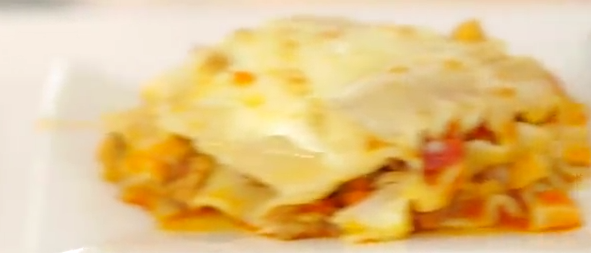
\includegraphics[scale=0.4]{Lasagna.png}
\end{center}


\end{document} 











